% %%%%%%%%%%%%%%%%%%%%%%%%%%%%%%%%%%%%%%%%%%%%%%%%%%%%%%%%%%%%%%%%%%%%%%
% Dummy Chapter:
% %%%%%%%%%%%%%%%%%%%%%%%%%%%%%%%%%%%%%%%%%%%%%%%%%%%%%%%%%%%%%%%%%%%%%%

% %%%%%%%%%%%%%%%%%%%%%%%%%%%%%%%%%%%%%%%%%%%%%%%%%%%%%%%%%%%%%%%%%%%%%%
% The Introduction:
% %%%%%%%%%%%%%%%%%%%%%%%%%%%%%%%%%%%%%%%%%%%%%%%%%%%%%%%%%%%%%%%%%%%%%%
\fancychapter{Architecture}
\label{cap:architecture}

This chapter gives an overview of the state of the art of Indoor positining solutions. The \acf{BLE}'s architecture and functionality is analyzed in section \ref{sec:ble}, while section \ref{sec:indoortech} overviews the other existing technologies. The most common techniques utilized for position computation along side examples which make use of them are explained in section \ref{sec:techniques}. Finnally on section \ref{sec:related} analyzes the most projects that had the most relevance in the field and the existing work related to \ac{BLE}.

\input{3.Chapter/1.requisites.tex}
\section{Generic Architecture} 
\label{sec:generic} 
 
 
The solution presented in this thesis was made with the objective of creating a generic indoor location system capable of being implemented and deployed using widely available technologies. Another important concept is the capability of allowing multiple different technologies on the same system to work seamlessly. The generic system's architecture is presented in figure ~\ref{fig:generic} and is divided in 4 parts: beacon, location server, map server and smartphone application.  
 
 
 
 
\begin{figure}[H] 
\centering 
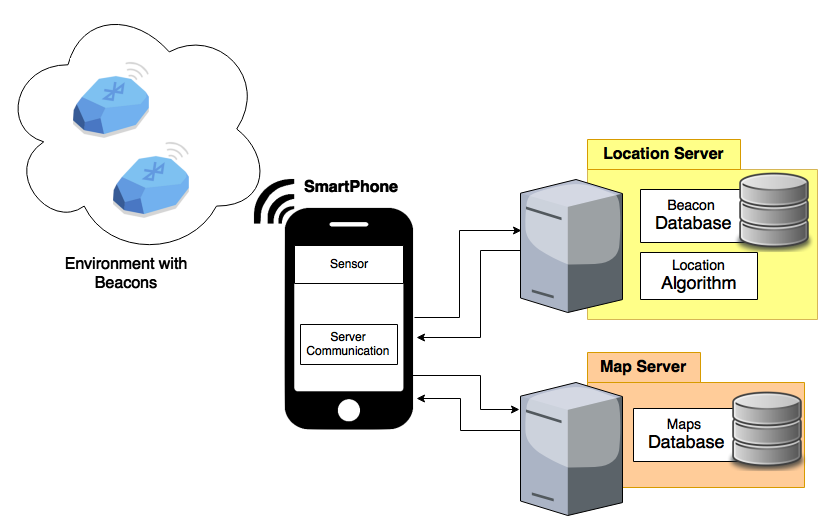
\includegraphics[width=1\linewidth]{3.Chapter/generic.png} 
\caption[Generic System's Architecture]{Generic System's Architecture} 
\label{fig:generic} 
\end{figure} 
 
 
The environment with beacons represents any form of element responsible for providing fixed reference points which are fundamental in calculating a user's position. A beacon needs to be compatible with the smartphone sensor, i.e. the device's sensors need to be able to capture the data. Using the previously presented technologies as examples, these beacons could be in fact BLE enabled beacons , Wi-Fi access points, LED lamps or even sound, with the data capturing being made through the smartphone's available antennas, camera or microphone respectfully. The beacon represents a position in the indoor environments and as such it needs to be uniquely identified, be it through its characteristics or associated information. In addition to these informations, each beacon needs to be assigned to a location server and be capable of handing over its information to the smartphone application.  
 
 
 
 
The location server is an external component where the information relative to the beacons utilised is stored. As such when a location request arrives from the smartphone, the received data can be translated into physical reference points which will later be used to compute the user's location. Once the location is obtained, two things are sent back to the smartphone: the calculated location and the address of the map server. 
 
 
The map server represents the architectural block responsible for providing the maps associated to the location of the user, location which was obtained through the location service on the application. The used map representation is up to the system, for as long as it is in accordance with the remaining parts of the system. This means that the location provided by the location server needs to be representable on the provided maps and capable of being comprehended by the smartphone application.  
 
 
The smartphone application is the central piece of this architecture. It is in charge of discovering and communicating with the beacons existent in its environment through its sensors. This communication process allows the smartphone to obtain information of its surrounding and to obtain the address of the location server that is associated to the connected beacon, in order to later forward this same information to it. Upon communicating with the location server, the application expects to get back information relative to its positions as well as the address of the map server that is to be contacted. Through that address, the application is capable of obtaining the map relative to its positions and display the result to the user. 
 
 
The presented architecture was structured in a way that it is scalable and allowed for interoperability. The idea behind this architecture is to let different indoor buildings use their own implementation of the system while a user with the associated smartphone application would be able to transit between buildings without changing configuration. This would be achieved through a common architecture that allowed for self-contained implementations to be accessed through a generic smartphone application. In order to analyse this assumption it is necessary to look back on the already analysed figure \ref{fig:choices}, located on section \ref{sec:int_motivation}, which represents the main components of an indoor systems. The architecture proposes an isolation of the algorithm and location representation, with the intention of having a more flexible system. By making the smartphone the central piece of communication, the beacons are required to be the ones providing the data for location calculation. Through a server dedicated to computing the location of an user, the system developers are allowed to use whichever algorithm they wish, since there is no dependency linked to the application.  
 
 
\subsection{Deployment environment} 
\label{subsec:deployment} 
 
 
In order to understand how a system based on this generic architecture, figure \ref{fig:generic}, has to be structured, it is relevant to analyse the system component's description and requirements that would allow it to be deployed.  
 
 
The smartphone service is the component that is in charge of communicating with both the beacons and the location server. This service is a software component of the smartphone application which is controlled by the app and is in charge of providing the user's location. Once a location is requested by the application, the service initiates discovery with nearby beacons through one of its sensors. A service is associated with one technology, as such if the application has to support more than one technology, multiple services should be implemented. This condition is fundamental since it allows the service to quickly tag the data with its associated technology, information which must be delivered to the location server. Once the beacon data has been collected, that data is forwarded to a server. Upon obtaining a location from the server, the service should forward the location to the app, which is responsible of later communicating with the map server. In terms of requirements, the service needs to have Wi-Fi or at least mobile network available for communicating with both the location and maps server, and access to the sensor required to communicate with the nearby beacon. In the case of BLE it would be the Bluetooth antenna while for QR it would be the camera. 
 
 
If one starts by analysing the beacons component, one can describe them as the reference points of the system which are in charge of providing nearby users with information relative to their surroundings. These beacons are available to the users and once contacted should make available to the smartphone the address of the its associated location server. Since the beacon only communicates with the smartphone, it isn't required to have any other communication capacity other than that specific to its technology. The communication between the smartphone and the beacon should include enough information to calculate the position. 
 
 
The Location server should have a database of all the beacons associated to it, each with its exact location of the map. This location is dependent on the method for location description chosen. The server should also be able to handle input from any of the supported technologies and apply the implemented algorithm, so that the user's location is obtained. From this description one can define the requirements of the location server as having stored the beacons that are associated it as well as their location. The location server must also be capable of communicating with the smartphone application, as well as be in accordance with the map server, achieved through providing location description that is the same as that present in the maps server. Assuming that all requirements are met, the location server should be capable of obtaining a location through its implemented location calculation algorithm. 
 
 
The Map server is responsible for providing the application with the maps that it has requested. The only decision concerning this server is the type of location description that is to be used and consequently the only requirement is that it has to be in accordance with the information on the location server. 
 
 
 
\cleardoublepage
